\section{Definizione del modello}
\begin{figure}[h]
    \centering
    \begin{tikzpicture}
        \pgftransparencygroup
        \nodes{\varphi_{0},\varphi_{0}}
        \endpgftransparencygroup
        \pgftransparencygroup
        \nodes{\varphi_{1},\varphi_{1},\varphi_{1}}
        \endpgftransparencygroup
        \pgftransparencygroup
        \hiddennodes{.,.,.}
        \endpgftransparencygroup
        \pgftransparencygroup
        \nodes{\varphi_{n},\varphi_{n}}
        \endpgftransparencygroup
        \pgftransparencygroup
        \brckt{1}{2}{0}{$\psi_{0}$}
        \endpgftransparencygroup
        \pgftransparencygroup
        \brckt{3}{5}{0}{$\psi_{1}$}
        \endpgftransparencygroup
        \pgftransparencygroup
        \brckt{9}{10}{0}{$\psi_{n}$}
        \endpgftransparencygroup
        \pgftransparencygroup
        \brckt{1}{10}{2}{$L$}
        \endpgftransparencygroup
    \end{tikzpicture}
    \caption{Rappresentazione della popolazione iniziale di cellule con i rispettivi
        valori di fluorescenza $\varphi_{i}$ tramite un array unidimensionale
        di lunghezza $L$}
    \label{fig:population-array}
\end{figure}
\begin{figure}[h]
\centering
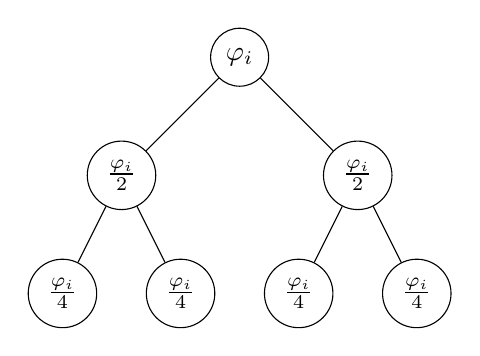
\begin{tikzpicture}[level/.style={sibling distance=30mm/#1}]
    \node [circle, draw] (a) {$\varphi_{i}$}
        child {
            node [circle,draw] (b) {$\frac{\varphi_{i}}{2}$}
                child {
                    node [circle,draw] (d) {$\frac{\varphi_{i}}{4}$}
                }
                child {
                    node [circle,draw] (e) {$\frac{\varphi_{i}}{4}$}
                }
        }
        child {
            node [circle,draw] (c) {$\frac{\varphi_{i}}{2}$}
                child {
                    node [circle,draw] (f) {$\frac{\varphi_{i}}{4}$}
                }
                child {
                    node [circle,draw] (g) {$\frac{\varphi_{i}}{4}$}
                }
        };
\end{tikzpicture}
\caption{Fenomeno di divisione cellulare rappresentato tramite albero
    binario bilanciato dove ogni nodo possiede un valore di fluorescenza
    $\varphi_{i}$ dimezzato rispetto al nodo precedente}
\label{fig:proliferation-tree}
\end{figure}
La simulazione del fenomeno prevede la creazione di una popolazione iniziale
di cellule basata su un istogramma fornito in input denominato $H(0)$
contenente coppie di valori ($\varphi_{i}, \psi_{i}$),
con $\varphi_{i} \in \R, \psi_{i} \in \N$ indicanti rispettivamente il
valore di fluorescenza rilevato dalle misurazioni in laboratorio e
la frequenza con il quale esso si presenta all'interno dei campioni analizzati.
\\
La popolazione iniziale di cellule, denominata $X_{0}$, è rappresentabile
tramite un array di
lunghezza $L$ pari alla seguente formula: 
$$L = \sum_{i=1}^{|\varphi|} \psi_{i}$$
$X_{0}$ è rappresentato in figura \ref{fig:population-array} dove si
può notare che ad ogni elemento
di un sottoinsieme di dimensione $\psi_{i}$ viene assegnato il corrispondente
valore di fluorescenza $\varphi_{i}$.
Il fenomeno di divisione cellulare è modellabile tramite un albero binario 
bilanciato
come mostrato in figura \ref{fig:proliferation-tree}, dove ogni nodo rappresenta
una cellula della popolazione con valore di fluorescenza $\varphi_{i}$
dimezzato rispetto alla cellula dalla quale ha avuto origine, infine ogni
ramo indica l'evento di proliferazione corrispondente.
$X_{0}$ dà origine ad un insieme di $L$ alberi di
divisione, le quali radici definiscono un insieme di primo livello di cellule
proliferanti e di conseguenza ogni livello successivo degli alberi rappresenterà
un nuovo stadio di proliferazione cellulare avente popolazione con numerosità
uguale a $L * 2^{i}$ con $i$ indicante il livello preso in considerazione.
Ne consegue che se il primo livello dell'albero corrisponde a $X_{0}$,
allora ad ogni livello successivo corrisponde un array $X_{n}$ i quali
elementi sono le nuove cellule ottenute dalla divisione cellulare avvenuta a 
partire da $X_{n-1}$.
In definitiva la totalità dei fenomeni di proliferazione è descritta da un
insieme di array, dove ognuno racchiude tutte e sole le cellule
corrispondenti ad uno specifico livello degli alberi di proliferazione generati
a partire da $X_{0}$.
